\documentclass[11pt,a4paper]{article}

\usepackage[margin=1in]{geometry}
\usepackage[T1]{fontenc}
\usepackage[utf8]{inputenc}
\usepackage{lmodern}
\usepackage{amsmath,amssymb,bm,mathtools}
\usepackage{booktabs}
\usepackage{graphicx}
\usepackage{longtable}
\usepackage{enumitem}
\usepackage{xcolor}
\usepackage{hyperref}
\usepackage{url}

\hypersetup{
  colorlinks=true,
  linkcolor=blue!50!black,
  citecolor=blue!50!black,
  urlcolor=blue!50!black
}

\setlength{\parindent}{0pt}
\setlength{\parskip}{0.45em}
\setlist[itemize]{leftmargin=1.4em,itemsep=0.15em,topsep=0.25em}
\setlist[enumerate]{leftmargin=1.6em,itemsep=0.15em,topsep=0.25em}

\newcommand{\dd}{\mathrm{d}}
\newcommand{\ii}{\mathrm{i}}
\newcommand{\ee}{\mathrm{e}}
\newcommand{\vpar}{v_{\parallel}}
\newcommand{\kperp}{k_{\perp}}
\newcommand{\bvec}{\bm b}
\newcommand{\Bvec}{\bm B}
\newcommand{\Evec}{\bm E}
\newcommand{\grad}{\nabla}
\newcommand{\avg}[1]{\left\langle #1 \right\rangle}
\newcommand{\fluxavg}[1]{\left\langle #1 \right\rangle_{\psi}}
\newcommand{\RHS}{\mathcal{R}}
\newcommand{\Dop}{\mathcal{D}}
\newcommand{\Jzero}{J_0}
\newcommand{\Gzero}{\Gamma_0}
\newcommand{\Lref}{R_{\mathrm{ref}}}
\newcommand{\vref}{v_{\mathrm{th,ref}}}
\newcommand{\rhoref}{\rho_{\mathrm{ref}}}
\newcommand{\crefpath}[1]{\path{#1}}
\DeclareMathOperator{\diag}{diag}
\DeclareMathOperator{\argmax}{arg\,max}

\title{Physical Model and Numerical Scheme for a Differentiable Flux-Tube Stellarator Gyrokinetic Solver}
\author{Mohsen Sadr}
\date{\today}

\begin{document}
\maketitle

\begin{abstract}
This document specifies the first implementation target for the project: a differentiable, local, flux-tube, linear electrostatic gyrokinetic solver for stellarator geometry.  The physics, normalization, signs, and benchmarks follow the published GKW model, the original GKW Fortran source, and the differentiable Gyaradax implementation.  The numerical target follows \path{task.tex}: Fourier discretization in the perpendicular directions and spectral discretization along the magnetic field and velocity-space coordinates.  GKW-style finite differences are retained as a fallback and parity backend.  Text is intentionally brief; equations, array contracts, numerical operators, and tests are written in enough detail to guide implementation in \path{src/}.
\end{abstract}

\tableofcontents

\section{Scope and Reference Hierarchy}

The first solver shall implement the collisionless linear electrostatic local gyrokinetic system in a stellarator flux tube.  The baseline electron model is adiabatic electrons with kinetic ions.  Kinetic electrons, nonlinear ExB dynamics, collisions, electromagnetic perturbations, rotation, and global radial effects are documented as extensions, not as the first implementation target.

When conventions are ambiguous, use the following order of authority.
\begin{enumerate}
  \item Published GKW paper: \path{papers/gkw/GKW.pdf}.
  \item Original GKW source: \path{relevant-codes/gkw/src/}.
  \item Searchable paper reconstruction: \path{papers/gkw/GKW_rebuilt.tex}.
  \item GKW sample cases: \path{relevant-codes/gkw/samples/}.
  \item Gyaradax JAX implementation and tests: \path{relevant-codes/gyaradax/}.
  \item DESC and stellarator optimization papers for Boozer geometry and design-loop coupling.
\end{enumerate}

The implementation must expose a pure residual
\begin{equation}
  \partial_t f = \RHS(f;\phi,\mathcal{G},p),
  \qquad
  \phi = \Phi(f;\mathcal{G},p),
  \label{eq:residual-contract}
\end{equation}
where \(f\) is the gyrocenter distribution perturbation, \(\phi\) is the electrostatic potential, \(\mathcal{G}\) is the flux-tube geometry, and \(p\) collects species, profile, grid, and solver parameters.  The residual is the central object for time stepping, eigenvalue solves, and automatic differentiation.

The primary discretization is:
\begin{equation}
  (x,y)\hbox{ Fourier}
  \quad+\quad
  z\hbox{ spectral}
  \quad+\quad
  (\vpar,\mu)\hbox{ spectral}.
  \label{eq:primary-discretization}
\end{equation}
Finite-difference stencils from GKW/Gyaradax are not the default target for new solver kernels.  They are a documented fallback for source-code parity, debugging, and convergence comparisons.

\subsection{GKW Source Crosswalk}

\begin{longtable}{p{0.31\textwidth}p{0.61\textwidth}}
\toprule
Reference file & Use in this project \\
\midrule
\path{linart.f90} & Main program flow and run sequencing. \\
\path{normalise.F90} & Normalization, growth-rate/frequency conventions. \\
\path{geom.F90} & Geometry, metric elements, drift tensors, circular and general geometry. \\
\path{mode.F90} & Fourier mode grids, radial/binormal mode labels, twist-and-shift connectivity. \\
\path{grid.F90}, \path{velocitygrid.F90} & Legacy grid sizes, velocity-space nodes, and weights for parity/fallback tests. \\
\path{components.F90} & Species parameters, Maxwellians, charges, masses, density and temperature ratios. \\
\path{functions.F90}, \path{specfun.f90} & Special functions used by Bessel and polarization factors. \\
\path{linear_terms.F90} & Linear gyrokinetic terms, Poisson/quasineutrality pieces, sign conventions. \\
\path{non_linear_terms.F90} & Future nonlinear ExB bracket, FFT/dealiasing, nonlinear timestep estimate. \\
\path{exp_integration.F90} & Explicit RK schemes, RHS assembly, field update flow. \\
\path{matdat.F90} & Matrix preparation, fallback stencil coefficients, linear timestep estimates. \\
\path{diagnostic.F90} & Growth rates, frequencies, fluxes, spectra, and output normalization. \\
\path{collisionop.F90}, \path{rotation.F90} & Future extensions beyond the first collisionless non-rotating baseline. \\
\bottomrule
\end{longtable}

\section{Normalization}

All implemented equations should use a dimensionless normalization close to GKW/Gyaradax.  Let \(\Lref\), \(B_{\mathrm{ref}}\), \(m_{\mathrm{ref}}\), \(T_{\mathrm{ref}}\), \(n_{\mathrm{ref}}\), and \(Z_{\mathrm{ref}}e\) be reference values.  Define
\begin{equation}
  \vref = \sqrt{\frac{2T_{\mathrm{ref}}}{m_{\mathrm{ref}}}},
  \qquad
  t_{\mathrm{ref}} = \frac{\Lref}{\vref},
  \qquad
  \rhoref = \frac{m_{\mathrm{ref}}\vref}{Z_{\mathrm{ref}} e B_{\mathrm{ref}}}.
\end{equation}
The dimensionless variables are
\begin{equation}
  \hat t = \frac{t}{t_{\mathrm{ref}}},
  \qquad
  \hat{\bm x} = \frac{\bm x}{\Lref},
  \qquad
  \hat B = \frac{B}{B_{\mathrm{ref}}},
  \qquad
  \hat \phi = \frac{Z_{\mathrm{ref}} e \phi}{T_{\mathrm{ref}}},
  \qquad
  \hat f_s = \frac{f_s}{n_{\mathrm{ref}}/\vref^3}.
\end{equation}
The hats are dropped below.  Species parameters are stored as
\begin{equation}
  \hat m_s = \frac{m_s}{m_{\mathrm{ref}}},
  \quad
  \hat Z_s = \frac{Z_s}{Z_{\mathrm{ref}}},
  \quad
  \hat T_s = \frac{T_s}{T_{\mathrm{ref}}},
  \quad
  \hat n_s = \frac{n_s}{n_{\mathrm{ref}}},
  \quad
  v_{\mathrm{th},s} = \sqrt{\frac{\hat T_s}{\hat m_s}}.
\end{equation}
The local profile gradients are dimensionless inverse scale lengths
\begin{equation}
  \omega_{n,s} = \frac{\Lref}{L_{n,s}}
  = -\Lref \frac{\dd \ln n_s}{\dd r},
  \qquad
  \omega_{T,s} = \frac{\Lref}{L_{T,s}}
  = -\Lref \frac{\dd \ln T_s}{\dd r}.
  \label{eq:profile-gradients}
\end{equation}
Implementation names should be close to Gyaradax/GKW: \(\omega_{n,s}\leftrightarrow\) \texttt{rln}, \(\omega_{T,s}\leftrightarrow\) \texttt{rlt}, \(\hat m_s\leftrightarrow\) \texttt{mas}, \(\hat Z_s\leftrightarrow\) \texttt{signz}, \(\hat T_s\leftrightarrow\) \texttt{tmp}, and \(\hat n_s\leftrightarrow\) \texttt{de}.

\section{Coordinates and Phase Space}

\subsection{Flux-tube coordinates}

Use a local field-aligned coordinate system
\begin{equation}
  (x,y,z) \equiv (\hbox{radial},\hbox{binormal},\hbox{parallel}),
  \qquad
  \Bvec = \grad \psi \times \grad \alpha,
  \label{eq:clebsch}
\end{equation}
where \(\psi\) labels the flux surface and \(\alpha\) labels a field line.  In Boozer angles \((\theta,\varphi)\), a standard choice is
\begin{equation}
  \alpha = \theta - \iota(\psi)\varphi - \alpha_0,
  \qquad
  \iota = \frac{1}{q}.
  \label{eq:alpha-boozer}
\end{equation}
The coordinate \(z\) parameterizes distance along the selected field line.  For compatibility with GKW/Gyaradax, a cell-centered grid on \(z\in[-n_{\mathrm{period}}+1/2,n_{\mathrm{period}}-1/2]\) is acceptable for analytic tests.  For stellarators, \(z\) may be Boozer toroidal angle, Boozer poloidal angle, or an arc-length-like coordinate, provided the geometry supplies \(\bvec\cdot\grad z\).

The Fourier representation in the perpendicular plane is
\begin{equation}
  h(x,y,z,\vpar,\mu,t)
  =
  \sum_{k_x,k_y} \hat h_{k_x,k_y}(z,\vpar,\mu,t)
  \exp\!\left[\ii(k_x x+k_y y)\right],
  \label{eq:fourier}
\end{equation}
with real-field Hermitian symmetry represented by a nonnegative \(k_y\) half spectrum.

\subsection{Phase-space state}

The evolved variable for species \(s\) is
\begin{equation}
  f_s = f_s(\vpar,\mu,z,k_x,k_y,t),
  \label{eq:state}
\end{equation}
where \(\mu = v_\perp^2/(2B)\) in physical variables and is represented on a positive grid.  The first implementation may use one kinetic ion species with adiabatic electrons:
\begin{equation}
  f \in \mathbb{C}^{N_{v}\times N_{\mu}\times N_z\times N_x\times N_y}.
\end{equation}
The multi-species extension adds a leading species axis:
\begin{equation}
  f \in \mathbb{C}^{N_s^{\mathrm{sp}}\times N_{v}\times N_{\mu}\times N_z\times N_x\times N_y}.
\end{equation}

\section{Geometry Required by the Solver}

At every \(z_j\), the solver needs a geometry object \(\mathcal{G}(z_j)\) that supplies enough information to form \(k_\perp^2\), parallel streaming, mirror force, ExB response, and magnetic drifts.  The minimal internal geometry contract is
\begin{equation}
  \mathcal{G} =
  \left\{
  B,\;
  F,\;
  G,\;
  E_y,\;
  D_x,D_y,\;
  g^{xx},g^{xy},g^{yy},\;
  w_z,\;
  \hbox{mode connectivity}
  \right\}.
  \label{eq:geometry-contract}
\end{equation}
This maps naturally to Gyaradax/GKW-style arrays:
\begin{center}
\begin{tabular}{ll}
\toprule
This document & Gyaradax/GKW-like name \\
\midrule
\(B(z)\) & \texttt{bn} \\
\(F(z)\), parallel streaming coefficient & \texttt{ffun} \\
\(G(z) = -B^{-1}\partial_z B\) up to coordinate factors & \texttt{gfun} \\
\(E_y(z)\), ExB/profile-drive coefficient & \texttt{efun} \\
\((D_x,D_y)(z)\), magnetic drift coefficients & \texttt{dfun[:,0:2]} \\
\((g^{yy},g^{xy},g^{xx})(z)\) & \texttt{little\_g[:,0:3]} \\
\(w_z\) & \texttt{ints} \\
\bottomrule
\end{tabular}
\end{center}

The perpendicular wavenumber is evaluated as
\begin{equation}
  \kperp^2(z;k_x,k_y)
  =
  k_x^2 g^{xx}(z)
  +2 k_x k_y g^{xy}(z)
  +k_y^2 g^{yy}(z).
  \label{eq:kperp}
\end{equation}
Numerically, enforce \(\kperp^2\ge 0\) up to a small tolerance.  Negative values beyond roundoff indicate an invalid metric or coordinate conversion.

\subsection{Stellarator geometry import}

The first imported-geometry interface uses \(\rho\) as the default radial
surface coordinate, interpreted as a minor-radius-like normalized label.  The
adapter may also carry metadata for \(\psi\) or \(x\), but the internal solver
contract uses the local radial coordinate \(x\) and stores the chosen source
coordinate as metadata.  Do not differentiate through changes of radial
coordinate convention.

For stellarator flux tubes, compute or load the following physical quantities along a field line:
\begin{equation}
\begin{split}
  \mathcal{G}_{\mathrm{phys}} =
  \{&
  B,\;
  \bvec\cdot\grad z,\;
  |\grad \psi|^2,\;
  |\grad \alpha|^2,\;
  \grad\psi\cdot\grad\alpha, \\
  &(\Bvec\times\grad B)\cdot\grad\psi,\;
  (\Bvec\times\grad B)\cdot\grad\alpha,\;
  (\bvec\times\bm\kappa)\cdot\grad\psi,\;
  (\bvec\times\bm\kappa)\cdot\grad\alpha
  \},
  \label{eq:stellarator-geometry}
\end{split}
\end{equation}
where \(\bm\kappa=\bvec\cdot\grad\bvec\).  The implementation should include an adapter
\begin{equation}
  \mathcal{G}_{\mathrm{phys}}
  \longmapsto
  \{B,F,G,E_y,D_x,D_y,g^{xx},g^{xy},g^{yy}\}
  \label{eq:geometry-adapter}
\end{equation}
with tests on analytic circular geometry before using DESC/Boozer equilibria.
The first supported import path is precomputed arrays on a sampled Boozer
field line.  DESC, SIMSOPT/Boozer objects, VMEC, or booz\_xform files should be
added as source adapters that produce the same precomputed physical-array
contract.

For coupling to DESC, the intended interface is array-based rather than a
refactor of DESC inside the gyrokinetic package.  DESC should solve or optimize
the MHD equilibrium and evaluate the flux-tube quantities in
\eqref{eq:stellarator-geometry} on the selected nodes \(z_i\):
\begin{equation}
  \mathcal{A}_{\mathrm{DESC}}
  \colon
  \{E_{\mathrm{DESC}},\rho,\alpha,z_i\}_{i=1}^{N_z}
  \longmapsto
  \left\{\mathcal{G}_{\mathrm{phys}}(z_i)\right\}_{i=1}^{N_z}.
  \label{eq:desc-array-adapter}
\end{equation}
The gyrokinetic solver then maps these arrays with
\eqref{eq:geometry-adapter}, builds the fixed-topology residual, and evaluates
the objective.  If DESC exposes JAX-compatible sensitivities of
\(\mathcal{G}_{\mathrm{phys}}\) with respect to equilibrium parameters \(p\),
the design gradient is assembled by the chain rule
\begin{equation}
  \frac{\partial \mathcal{J}}{\partial p}
  =
  \sum_i
  \frac{\partial \mathcal{J}}{\partial \mathcal{G}_{\mathrm{phys}}(z_i)}
  \frac{\partial \mathcal{G}_{\mathrm{phys}}(z_i)}{\partial p}.
  \label{eq:desc-chain-rule}
\end{equation}
This keeps file I/O, equilibrium solves, and any remeshing outside the
time-advance kernels while preserving differentiation through continuous
geometry arrays.

\subsection{Magnetic drift coefficient}

Use a geometry-factorized magnetic drift frequency
\begin{equation}
  \omega_{d,s}(z,\vpar,\mu,k_x,k_y)
  =
  \frac{v_\parallel^2+\mu B(z)}{Z_s}
  \left[
    k_x D_x(z)+k_y D_y(z)
  \right],
  \label{eq:omega-d}
\end{equation}
where all dimensional constants are absorbed into the normalization and the geometry coefficients.  This is the first implementation form because it matches the Gyaradax/GKW coefficient structure and is easy to test.  Later, if curvature and grad-\(B\) drifts are separated, retain \eqref{eq:omega-d} as the assembled operator interface.

\section{Maxwellian, FLR Factors, and Polarization}

The normalized background Maxwellian is
\begin{equation}
  F_{M,s}(\vpar,\mu,z)
  =
  \frac{n_s}{(\pi T_s)^{3/2}}
  \exp\!\left[
    -\frac{\vpar^2+2\mu B(z)}{T_s}
  \right],
  \label{eq:maxwellian}
\end{equation}
where \(T_s\) and \(n_s\) are normalized species values.  Define the normalized particle energy and thermodynamic drive factor
\begin{equation}
  \mathcal{E}_s(\vpar,\mu,z)
  =
  \frac{\vpar^2+2\mu B(z)}{T_s},
  \qquad
  \Xi_s
  =
  \omega_{n,s}
  +
  \omega_{T,s}\left(\mathcal{E}_s-\frac{3}{2}\right).
  \label{eq:drive-factor}
\end{equation}

The gyroaverage of \(\phi\) is algebraic in Fourier space:
\begin{equation}
  \avg{\phi}_s
  =
  \Jzero(a_s)\phi,
  \qquad
  a_s
  =
  \frac{m_s v_{\mathrm{th},s}}{|Z_s|}
  \frac{\kperp}{B}
  \sqrt{2\mu B}.
  \label{eq:j0}
\end{equation}
The polarization factor uses
\begin{equation}
  b_s
  =
  \frac{1}{2}
  \left(
    \frac{m_s v_{\mathrm{th},s}}{Z_s}
    \frac{\kperp}{B}
  \right)^2,
  \qquad
  \Gzero(b_s) = I_0(b_s)\ee^{-b_s}.
  \label{eq:gamma0}
\end{equation}
Implementation detail: use a numerically stable exponentially scaled Bessel function for \(\Gzero\), e.g. \texttt{i0e}, and test the small-\(b\) limit \(\Gzero(b)=1-b+\mathcal{O}(b^2)\).

\section{Linear Electrostatic Gyrokinetic Model}

The first implementation evolves the collisionless linear electrostatic system
\begin{equation}
  \partial_t f_s
  =
  \RHS_s(f_s,\phi)
  =
  \mathcal{T}_{I,s}
  +\mathcal{T}_{II,s}
  +\mathcal{T}_{IV,s}
  +\mathcal{T}_{V,s}
  +\mathcal{T}_{VII,s}
  +\mathcal{T}_{VIII,s}
  +\Dop_s.
  \label{eq:linear-rhs}
\end{equation}
Term numbers follow the GKW/Gyaradax convention.  Term III, the nonlinear ExB term, is omitted in the linear baseline and documented in Section~\ref{sec:nonlinear-extension}.

Let
\begin{equation}
  a_{\parallel,s}(z,\vpar)=v_{\mathrm{th},s}F(z)\vpar,
  \qquad
  a_{\mu,s}(z,\mu)=v_{\mathrm{th},s}\mu B(z)G(z).
  \label{eq:adv-speeds}
\end{equation}
Then the six active linear terms are:
\begin{align}
  \mathcal{T}_{I,s}
  &=
  -a_{\parallel,s}\,\partial_z f_s,
  &&\hbox{parallel streaming,}
  \label{eq:term-I}
  \\
  \mathcal{T}_{II,s}
  &=
  -\ii\,\omega_{d,s}\,f_s,
  &&\hbox{magnetic drift advection,}
  \label{eq:term-II}
  \\
  \mathcal{T}_{IV,s}
  &=
  a_{\mu,s}\,\partial_{\vpar} f_s,
  &&\hbox{mirror force/trapping,}
  \label{eq:term-IV}
  \\
  \mathcal{T}_{V,s}
  &=
  \ii\,k_y\,E_y(z)\,
  J_{0,s}\phi\,
  F_{M,s}\,\Xi_s,
  &&\hbox{equilibrium-gradient drive,}
  \label{eq:term-V}
  \\
  \mathcal{T}_{VII,s}
  &=
  -\frac{Z_s}{T_s}\,
  a_{\parallel,s}\,
  F_{M,s}\,
  \partial_z(J_{0,s}\phi),
  &&\hbox{parallel field drive,}
  \label{eq:term-VII}
  \\
  \mathcal{T}_{VIII,s}
  &=
  -\frac{Z_s}{T_s}\,
  \ii\,\omega_{d,s}\,
  F_{M,s}\,
  J_{0,s}\phi,
  &&\hbox{drift field drive.}
  \label{eq:term-VIII}
\end{align}
All products are pointwise over the discrete phase-space grid after broadcasting over species, velocity, field-line, and Fourier axes.

\subsection{Dissipation}

The baseline solver includes only numerical dissipation:
\begin{equation}
  \Dop_s
  =
  \Dop_{z,s}
  +\Dop_{v_\parallel,s}
  +\Dop_{\perp,s}.
  \label{eq:diss-total}
\end{equation}
For the spectral backend, use modal filtering or modal damping.  In a coordinate
\(\xi\in\{z,\vpar,\mu\}\),
\begin{equation}
  \Dop_{\xi,s} f_s
  =
  -\nu_\xi
  T_\xi^{-1}
  \diag\left[
    \left(\frac{r}{r_{\max}}\right)^{p_\xi}
  \right]
  T_\xi f_s,
  \qquad
  r=0,\ldots,r_{\max},
  \label{eq:spectral-diss}
\end{equation}
where \(T_\xi\) is the Fourier or Chebyshev modal transform.  Set
\(\nu_\xi=0\) by default.  GKW-style fourth-order damping is used only in the
finite-difference fallback backend.

The perpendicular directions remain Fourier, so perpendicular hyper-dissipation is
\begin{align}
  \Dop_{\perp,s} f_s
  &=
  -\left[
    \nu_x\left(\frac{|k_x|}{k_{x,\max}}\right)^{p_x}
    +
    \nu_y\left(\frac{|k_y|}{k_{y,\max}}\right)^{p_y}
  \right]f_s,
  \label{eq:perp-diss}
  \\
  p_x,p_y&=
  \begin{cases}
    4, & \nu_x,\nu_y \ge 0,\\
    2, & \nu_x,\nu_y < 0\quad \hbox{(GKW-style option).}
  \end{cases}
\end{align}
For the first implementation, set default \(\nu_x=\nu_y=0\) unless a benchmark specifies otherwise.  This avoids accidental damping of Rosenbluth-Hinton and linear ITG benchmarks.

\section{Quasineutrality}

\subsection{Adiabatic electrons}

For ion species \(i\) with adiabatic electrons, solve quasineutrality independently at each \((z,k_x,k_y)\):
\begin{equation}
  \phi
  =
  -
  \frac{
    \displaystyle
    \sum_i
    Z_i n_i
    \int \dd\vpar\,\dd\mu\,
    B\,J_{0,i} f_i
  }{
    \displaystyle
    \sum_i
    \frac{Z_i^2 n_i}{T_i}
    \left[\Gamma_{0,i}-1\right]
    -
    \frac{n_e}{T_e}
  }.
  \label{eq:phi-adiabatic}
\end{equation}
The discrete numerator uses the velocity weights \(w_v,w_\mu\):
\begin{equation}
  N_i(z,k_x,k_y)
  =
  Z_i n_i
  \sum_{\ell,m}
  w_{v,\ell} w_{\mu,m}
  B(z)\,
  J_{0,i}(\ell,m,z,k_x,k_y)
  f_i(\ell,m,z,k_x,k_y).
  \label{eq:phi-numerator-discrete}
\end{equation}

For the zonal mode \(k_y=0\), GKW/Gyaradax apply a flux-surface correction to the adiabatic response.  The implementation must keep this as a separately tested path.  A practical contract is:
\begin{equation}
  \phi_{k_y=0}
  =
  \Phi_{\mathrm{local}}(f)
  +
  \Phi_{\mathrm{zf\ correction}}(f),
  \label{eq:zonal-correction-contract}
\end{equation}
where \(\Phi_{\mathrm{zf\ correction}}\) is matched against \path{linear_terms.F90} routines \path{poisson_dia} and \path{poisson_zf} and against Gyaradax tests.

\subsection{Kinetic-electron extension}

For fully kinetic species, use
\begin{equation}
  \phi
  =
  -
  \frac{
    \displaystyle
    \sum_s
    Z_s n_s
    \int \dd\vpar\,\dd\mu\,
    B\,J_{0,s} f_s
  }{
    \displaystyle
    \sum_s
    \frac{Z_s^2 n_s}{T_s}
    \left[\Gamma_{0,s}-1\right]
  }.
  \label{eq:phi-kinetic}
\end{equation}
The zero-denominator zonal/constant mode must be regularized explicitly and tested.  This path is not required before the adiabatic baseline passes tests.

\section{Discrete Grids and Operators}

The target backend is spectral in all non-perpendicular coordinates.  Production kernels should therefore be written in terms of precomputed spectral quadrature weights and differentiation matrices.  A finite-difference backend may implement the same public interface for GKW parity and fallback convergence studies.

\subsection{Velocity-space spectral collocation}

The first spectral velocity backend should keep the finite velocity box used by GKW-style benchmarks, but replace uniform finite differences with Chebyshev--Lobatto collocation.  Let
\begin{equation}
  \xi_\ell = -\cos\frac{\pi\ell}{N_v-1},
  \qquad
  v_{\parallel,\ell}=v_{\max}\xi_\ell,
  \qquad
  \ell=0,\ldots,N_v-1,
  \label{eq:vpar-cheb-grid}
\end{equation}
and
\begin{equation}
  \eta_m=\frac{1-\cos\frac{\pi m}{N_\mu-1}}{2},
  \qquad
  \mu_m=\mu_{\max}\eta_m,
  \qquad
  m=0,\ldots,N_\mu-1.
  \label{eq:mu-cheb-grid}
\end{equation}
Let \(W^C_N\) and \(D^C_N\) denote Clenshaw--Curtis quadrature weights and the Chebyshev--Lobatto first-derivative matrix on \([-1,1]\).  The physical weights and derivative matrices are
\begin{equation}
  w_{v,\ell}=v_{\max} W^C_{N_v,\ell},
  \qquad
  w_{\mu,m}=\mu_{\max} W^{C,[0,1]}_{N_\mu,m},
  \qquad
  D_{v_\parallel}=\frac{1}{v_{\max}}D^C_{N_v},
  \qquad
  D_\mu=\frac{1}{\mu_{\max}}D^{C,[0,1]}_{N_\mu}.
  \label{eq:velocity-spectral-ops}
\end{equation}
Here \(W^{C,[0,1]}\) and \(D^{C,[0,1]}\) are the mapped weights and derivative matrix on \([0,1]\).  Velocity integrals use
\begin{equation}
  \int_{-v_{\max}}^{v_{\max}}\dd\vpar
  \int_0^{\mu_{\max}}\dd\mu\,
  B(z)\,g(\vpar,\mu,z)
  \approx
  B(z)
  \sum_{\ell,m} w_{v,\ell}w_{\mu,m}
  g_{\ell m}(z).
  \label{eq:velocity-spectral-quadrature}
\end{equation}
The gyrophase factor is absorbed into the chosen normalization; if a benchmark requires an explicit \(2\pi\), it should enter the documented velocity measure, not an individual physics term.  Hermite--Laguerre velocity bases are a later optimization path, not the first backend.

\subsection{Parallel spectral grid}

The parallel coordinate \(z\) is the chosen field-line parameter.  For a closed mode chain, use Fourier collocation along the concatenated connected coordinate:
\begin{equation}
  z_j=z_0+\frac{jL_z}{N_z},
  \qquad
  q_r=\frac{2\pi}{L_z}
  \begin{cases}
    r, & 0\le r\le N_z/2,\\
    r-N_z, & N_z/2<r<N_z,
  \end{cases}
  \label{eq:z-fourier-grid}
\end{equation}
and
\begin{equation}
  D_z = F_z^{-1}\diag(\ii q_r)F_z,
  \qquad
  w_{z,j}=L_z/N_z.
  \label{eq:z-fourier-derivative}
\end{equation}
Here \(F_z\) is the discrete Fourier transform along the connected field-line chain.  For an open or non-closing chain, use Chebyshev--Lobatto collocation on the finite interval and the corresponding derivative matrix.  In both cases the streaming operator is \(a_{\parallel,s}D_z f_s\); the geometry object supplies \(\bvec\cdot\grad z\), metric factors, and quadrature weights for the chosen coordinate.

For imported stellarator geometry, interpolate or evaluate \(B\), metric terms, and drift coefficients on the same spectral \(z\) nodes.  Do not hide the quadrature rule in the RHS; store \(z_j\), \(w_{z,j}\), \(D_z\), and any modal transform needed by filters in the geometry/precompute object.

\subsection{Fourier grids}

The \(k_y\) grid is a nonnegative half spectrum:
\begin{equation}
  k_{y,n} = n\Delta k_y,\qquad n=0,\ldots,N_y-1.
  \label{eq:ky-grid}
\end{equation}
The \(k_x\) grid is centered:
\begin{equation}
  k_{x,m} = (m-m_0)\Delta k_x,\qquad m=0,\ldots,N_x-1,
  \label{eq:kx-grid}
\end{equation}
where \(m_0\) indexes \(k_x=0\).  In single-mode linear runs, \(N_x=1\) and \(k_x=0\) is allowed.

Parseval weights for the \(k_y\) half spectrum are
\begin{equation}
  P(k_y)=
  \begin{cases}
    1, & k_y=0,\\
    2, & k_y>0.
  \end{cases}
  \label{eq:parseval}
\end{equation}

\subsection{Twist-and-shift connectivity}

At a parallel boundary, nonzonal modes connect to a shifted radial wavenumber.  Represent this with integer maps
\begin{equation}
  \mathrm{ixplus}(m,n),\qquad
  \mathrm{ixminus}(m,n),
  \label{eq:ixmaps}
\end{equation}
where invalid entries denote an open end of a connected mode chain.  For axisymmetric tests, the shift should reproduce GKW mode-box behavior.  For stellarators, compute the shift from the field-line twist:
\begin{equation}
  k_x^{+}
  =
  k_x + k_y\,\Delta_{\mathrm{twist}},
  \qquad
  \Delta_{\mathrm{twist}}
  =
  \left.
  \frac{\partial \alpha_{\mathrm{end}}}{\partial x}
  \right|_{\psi_0}
  -
  \left.
  \frac{\partial \alpha_{\mathrm{start}}}{\partial x}
  \right|_{\psi_0},
  \label{eq:twist-shift-general}
\end{equation}
then choose \(\Delta k_x\) so the shifted mode lands on an integer grid index when possible.  The continuous twist can be differentiable, but the integer connectivity maps are static topology and must not be differentiated.

\subsection{Spectral derivative contract}

All derivative-using RHS terms should call backend operators:
\begin{equation}
  \partial_z f \mapsto D_z f,
  \qquad
  \partial_{\vpar} f \mapsto D_{v_\parallel} f,
  \qquad
  \partial_\mu f \mapsto D_\mu f.
  \label{eq:spectral-derivative-contract}
\end{equation}
The implementation may store nodal-to-modal transforms \(T_\xi\) for filtering and diagnostics:
\begin{equation}
  \widehat f^{(\xi)} = T_\xi f,
  \qquad
  f = T_\xi^{-1}\widehat f^{(\xi)}.
  \label{eq:modal-transform}
\end{equation}
For smooth manufactured functions, derivative tests should demonstrate spectral convergence until floating-point or interpolation error dominates.  On nonsmooth or open-boundary tests, the code should still converge monotonically and the finite-difference backend provides a useful sanity check.

\subsection{GKW finite-difference fallback}

The following GKW/Gyaradax-style formulas are fallback operators, not the primary target discretization from \path{task.tex}.  They are useful for parity tests against the original implementation and for debugging spectral boundary behavior.

Interior fourth-order centered first derivative:
\begin{equation}
  (\partial_\xi f)_j
  =
  \frac{
    f_{j-2}-8f_{j-1}+8f_{j+1}-f_{j+2}
  }{12\Delta \xi}
  +\mathcal{O}(\Delta\xi^4).
  \label{eq:d1-centered}
\end{equation}
Interior fourth derivative stencil:
\begin{equation}
  (\partial_\xi^4 f)_j
  =
  \frac{
    f_{j-2}-4f_{j-1}+6f_j-4f_{j+1}+f_{j+2}
  }{\Delta\xi^4}
  +\mathcal{O}(\Delta\xi^2).
  \label{eq:d4-centered}
\end{equation}

The fallback parallel streaming operator uses sign-dependent upwinding.  Boundary stencils follow GKW/Gyaradax.  The implementation should store dimensionless stencil tables
\begin{equation}
  S_{z,+}^{(1)},\quad S_{z,-}^{(1)},\quad
  S_{z,+}^{(4)},\quad S_{z,-}^{(4)}
  \label{eq:stencil-tables}
\end{equation}
and select them by \(\operatorname{sign}(a_{\parallel,s})\).  At a boundary, a stencil point outside the \(z\)-domain is resolved with \(\mathrm{ixplus}\) or \(\mathrm{ixminus}\); if no connected mode exists, the point is treated with the chosen open-boundary rule.

For the fallback mirror term in \(v_\parallel\), use the centered fourth-order derivative in the interior and zero-padding/no-flux style boundary behavior, matching GKW velocity-space conventions.  Every derivative routine must have manufactured-solution tests in both spectral and fallback modes.

\section{Residual Assembly and Precomputation}

\subsection{Precomputed coefficient arrays}

Before a time loop or eigenvalue solve, construct a precompute object
\begin{equation}
  \mathcal{P} =
  \left\{
  \begin{array}{l}
  J_{0,s},\Gamma_{0,s},F_{M,s},\Xi_s,\omega_{d,s},\\
  a_{\parallel,s},a_{\mu,s},\\
  D_z,D_{v_\parallel},D_\mu,\quad
  T_z,T_{v_\parallel},T_\mu,\\
  \hbox{fallback stencil tables},\\
  \hbox{phi weights},\quad
  \hbox{diagnostic weights}
  \end{array}
  \right\}.
  \label{eq:precompute}
\end{equation}
Shapes for the adiabatic single-species path should be
\begin{equation}
\begin{array}{ll}
f: & (N_v,N_\mu,N_z,N_x,N_y),\\
\phi: & (N_z,N_x,N_y),\\
\Jzero,F_M,\omega_d: & (N_v,N_\mu,N_z,N_x,N_y),\\
a_\parallel,a_\mu: & (N_v,N_\mu,N_z,1,1).
\end{array}
\end{equation}
Multi-species arrays add a leading species axis.

\subsection{Public solver interfaces}

The core interfaces should be pure functions:
\begin{align}
  \phi &= \texttt{calculate\_phi}(f,\mathcal{G},p,\mathcal{P}),
  \label{eq:api-phi}
  \\
  r &= \texttt{linear\_residual}(f,\phi,\mathcal{G},p,\mathcal{P}),
  \label{eq:api-residual}
  \\
  f^{n+1} &= \texttt{rk4\_step}(f^n,\mathcal{G},p,\mathcal{P}).
  \label{eq:api-rk4}
\end{align}
No file I/O, Python-side mutation, random initialization, or diagnostic printing belongs inside these functions.  This keeps the residual JIT-compatible and differentiable.

\section{Time Integration and Linear Growth Rates}

\subsection{RK4}

The baseline time integrator is explicit fourth-order Runge--Kutta:
\begin{align}
  k_1 &= \RHS(f^n),\\
  k_2 &= \RHS(f^n+\tfrac{1}{2}\Delta t\,k_1),\\
  k_3 &= \RHS(f^n+\tfrac{1}{2}\Delta t\,k_2),\\
  k_4 &= \RHS(f^n+\Delta t\,k_3),\\
  f^{n+1} &= f^n + \frac{\Delta t}{6}(k_1+2k_2+2k_3+k_4).
  \label{eq:rk4}
\end{align}
Each RHS evaluation recomputes \(\phi=\Phi(f)\).  Multi-step runs should use a scan-style loop so that JAX can compile the full step block.

\subsection{Timestep estimate}

Use fixed \(\Delta t\) first.  Add adaptive estimates after the fixed-step solver passes benchmarks.  For the spectral backend, estimate the explicit stability limit using operator radii:
\begin{equation}
  \rho_1 =
  \rho\!\left(a_\parallel D_z+a_\mu D_\mu\right),
  \qquad
  \rho_{\mathrm{diss}} =
  \rho\!\left(\Dop_z+\Dop_{v_\parallel}+\Dop_\mu+\Dop_\perp\right),
  \label{eq:spectral-radii}
\end{equation}
where \(\rho(\cdot)\) is either an inexpensive power-iteration estimate or an upper bound from row sums on small grids.  A practical RK4 estimate is
\begin{equation}
  \Delta t_{\mathrm{spec}}
  =
  c_{\mathrm{safety}}
  \min\left(
    \frac{2.4}{\max(\rho_1,\epsilon)},
    \frac{2.4}{\max(\rho_{\mathrm{diss}},\epsilon)}
  \right).
  \label{eq:dtspec}
\end{equation}

The finite-difference fallback may also expose the GKW-compatible linear estimate
\begin{equation}
  \Delta t_{\mathrm{lin}}
  =
  \frac{c_{\mathrm{safety}}}
  {
    \max\left[
      40,\;
      \frac{t_1}{2.4},\;
      \frac{t_4}{2.4},\;
      \frac{t_{\mathrm{field}}}{2.4}
    \right]
  },
  \label{eq:dtlin}
\end{equation}
with
\begin{align}
  t_1 &=
  \max\left(
    c_{z,1}\frac{\max|a_\parallel|}{\Delta z},
    c_{v,1}\frac{\max|a_\mu|}{\Delta v}
  \right),
  \label{eq:t1}
  \\
  t_4 &=
  \max\left(
    c_{z,4}\nu_z\frac{\max|a_\parallel|}{\Delta z},
    c_{v,4}\nu_v\frac{\max|a_\mu|}{\Delta v}
  \right).
  \label{eq:t4}
\end{align}
Here \(2.4\) is the RK4 stability-boundary factor used in GKW/Gyaradax notes.  \(t_{\mathrm{field}}\) is needed mainly for kinetic electrons and can be zero in the adiabatic baseline.  The effective timestep is
\begin{equation}
  \Delta t
  =
  \min(\Delta t_{\mathrm{input}},\Delta t_{\mathrm{spec}},\Delta t_{\mathrm{lin}},\Delta t_{\mathrm{NL}}),
  \label{eq:dteff}
\end{equation}
where \(\Delta t_{\mathrm{lin}}\) is ignored unless the fallback backend is active, and \(\Delta t_{\mathrm{NL}}\) is relevant only after the nonlinear ExB term is implemented.

\subsection{Mode amplitude, growth rate, and frequency}

Let \(\mathcal{C}(k_y)\) be the connected \(k_x\)-chain containing \(k_x=0\).  Define the per-\(k_y\) potential amplitude
\begin{equation}
  A(k_y,t)
  =
  \left[
    \sum_{z} w_z
    \sum_{k_x\in\mathcal{C}(k_y)}
    |\phi(z,k_x,k_y,t)|^2
  \right]^{1/2}.
  \label{eq:mode-amplitude}
\end{equation}
Over a diagnostic window \([t_a,t_b]\),
\begin{equation}
  \gamma(k_y)
  =
  \frac{\log A(k_y,t_b)-\log A(k_y,t_a)}{t_b-t_a}.
  \label{eq:growth-rate}
\end{equation}
A robust real-frequency estimator is the phase rotation of the complex mode:
\begin{equation}
  \omega(k_y)
  =
  -\frac{1}{t_b-t_a}
  \arg
  \left[
    \sum_z w_z
    \sum_{k_x\in\mathcal{C}(k_y)}
    \phi^*(z,k_x,k_y,t_a)\phi(z,k_x,k_y,t_b)
  \right].
  \label{eq:frequency}
\end{equation}
In linear initial-value runs, normalize each active \(k_y\) after each diagnostic window:
\begin{equation}
  f_s(\cdots,k_y) \leftarrow
  \frac{f_s(\cdots,k_y)}{\max(A(k_y),\epsilon_A)}.
  \label{eq:linear-normalization}
\end{equation}
Store the accumulated normalization factor so diagnostics remain physically interpretable.

\section{Fluxes and Quasilinear Objective}

The immediate optimization objective is not nonlinear heat flux, but a differentiable linear proxy.  For each \(k_y\), define a mode-structure weighted perpendicular scale
\begin{equation}
  \avg{\kperp^2}_{k_y}
  =
  \frac{
    \displaystyle
    \sum_z w_z
    \sum_{k_x\in\mathcal{C}(k_y)}
    \kperp^2(z,k_x,k_y)|\phi(z,k_x,k_y)|^2
  }{
    \displaystyle
    \sum_z w_z
    \sum_{k_x\in\mathcal{C}(k_y)}
    |\phi(z,k_x,k_y)|^2+\epsilon_A
  }.
  \label{eq:kperp-average}
\end{equation}
The first quasilinear proxy is
\begin{equation}
  Q_{\mathrm{QL}}
  =
  \sum_{k_y>0}
  W(k_y)
  \frac{\max(\gamma(k_y),0)}{\avg{\kperp^2}_{k_y}+\epsilon_k}.
  \label{eq:ql-proxy}
\end{equation}
For smooth reverse-mode differentiation, replace \(\max(\gamma,0)\) by a softplus if needed:
\begin{equation}
  \max(\gamma,0)
  \approx
  \tau\log\left(1+\ee^{\gamma/\tau}\right).
  \label{eq:softplus-growth}
\end{equation}
This objective matches the spirit of direct microstability optimization while remaining cheap enough for early design-loop tests.

\section{Differentiability Contract}

The following quantities should be differentiable:
\begin{itemize}
  \item continuous geometry arrays \(B,F,G,E_y,D_x,D_y,g^{xx},g^{xy},g^{yy}\);
  \item profile gradients \(\omega_n,\omega_T\);
  \item species parameters where physically meaningful;
  \item scalar geometry knobs in analytic tests, e.g. \(q,\hat s,\epsilon\);
  \item objective functions \(A,\gamma,\omega,Q_{\mathrm{QL}}\) through a fixed number of time steps.
\end{itemize}
The following quantities are static/non-differentiable:
\begin{itemize}
  \item grid sizes;
  \item integer mode labels and connectivity maps;
  \item branch choices for topology;
  \item file I/O and equilibrium loading;
  \item random initialization keys.
\end{itemize}
For stellarator optimization, a differentiable equilibrium code may provide geometry arrays and their sensitivities.  The gyrokinetic solver should not require differentiating through an integer remeshing or topology change.
In the present implementation, imported DESC-style arrays are accepted as a
\texttt{desc} geometry model in the single-surface objective; the direct DESC object
reader remains a source-adapter task rather than a solver-core dependency.

\section{Current Reduced Optimization Results}
\label{sec:reduced-optimization-results}

This section records the first end-to-end optimization demonstrations produced
by the current implementation.  These are reduced solver plumbing tests, not
validated physical design results.  Their purpose is to show that the
linear residual, adiabatic field solve, RK4 initial-value objective, and
reverse-mode derivatives can be combined into a fixed-topology optimization
loop.

\subsection{Optimization problem}

For a vector of differentiable knobs
\begin{equation}
  u =
  \left(
    q,\hat s,\epsilon,\rho,\alpha,
    R/L_n,R/L_T,
    \beta,\beta',
    c_1,c_2,\ldots
  \right),
  \label{eq:optimization-knobs}
\end{equation}
the code evaluates a scalar objective
\begin{equation}
  J(u)
  =
  \mathcal{J}
  \left[
    \gamma(k_y;u),
    \omega(k_y;u),
    Q_{\mathrm{QL}}(u),
    \phi(z,k_x,k_y;u)
  \right],
  \qquad
  \frac{\partial J}{\partial u}
  =
  \mathrm{AD}\left[J(u)\right],
  \label{eq:optimization-objective}
\end{equation}
where the reduced examples choose a scalar residual \(r(u)\) from either a
selected nonzonal growth rate or the maximum nonzonal growth rate.  The
optimized cost is the zero-target least-squares objective
\begin{equation}
  J(u) = \frac{1}{2}\left|r(u)\right|^2,
  \qquad
  r(u) =
  \begin{cases}
    \gamma(k_y;u), & \text{selected-mode cases},\\
    \max_{k_y>0}\gamma(k_y;u), & \text{max-growth case}.
  \end{cases}
  \label{eq:optimization-zero-target-cost}
\end{equation}
The optimization update used for the figures is plain gradient descent,
\begin{equation}
  u^{(m+1)} = \Pi\!\left(u^{(m)}-\eta \nabla_u J(u^{(m)})\right),
  \label{eq:optimization-update}
\end{equation}
where \(\Pi\) only enforces positivity of \(q,\epsilon,n,T\).  The coefficients
\(c_i\) are low-amplitude toy equilibrium coefficients that modulate analytic
circular geometry.  They are included to exercise the same differentiable API
that later Boozer/DESC geometry coefficients will use.

\subsection{Reduced simulation setup}

All three examples use the same small fixed-topology linear electrostatic run:
\begin{itemize}
  \item one kinetic ion species and adiabatic electrons;
  \item analytic circular flux-tube geometry;
  \item Chebyshev--Lobatto velocity grids with \(N_{v_\parallel}=3\) and \(N_\mu=3\);
  \item periodic spectral parallel grid with \(N_z=5\);
  \item centered radial Fourier grid \(k_x\in\{-0.5,0,0.5\}\);
  \item endpoint-only RK4 integration with \(\Delta t=0.01\) and two steps per objective evaluation;
  \item deterministic complex initial condition
  \[
    f_0 = 10^{-2}\left[\cos(I/6)+\ii\sin(I/8)\right],
  \]
  where \(I\) is the flattened phase-space index reshaped onto
  \((v_\parallel,\mu,z,k_x,k_y)\).
\end{itemize}
The example data and figures are generated by
\begin{equation}
  \texttt{uv run --extra dev python examples/generate\_optimization\_figures.py}.
  \label{eq:figure-generation-command}
\end{equation}

\begin{table}[htbp]
\centering
\small
\setlength{\tabcolsep}{3pt}
\begin{tabular}{p{0.07\textwidth}p{0.18\textwidth}p{0.18\textwidth}p{0.34\textwidth}p{0.10\textwidth}}
\toprule
Case & \(k_y\rho_{\mathrm{ref}}\) grid & Objective \(J\) & Initial geometry/profile & Step size \(\eta\) \\
\midrule
A & \(\{0,0.35\}\) & \(\frac12|\gamma(k_y=0.35)|^2\) & \(q=1.25,\hat s=0.45,R/L_T=2.10,R/L_n=0.80\) & \(10^{-3}\) \\
B & \(\{0,0.25,0.50\}\) & \(\frac12|\gamma(k_y=0.50)|^2\) & \(q=1.35,\hat s=0.65,R/L_T=2.49,R/L_n=0.80\) & \(10^{-3}\) \\
C & \(\{0,0.25,0.50\}\) & \(\frac12|\max_{k_y>0}\gamma(k_y)|^2\) & \(q=1.45,\hat s=0.75,R/L_T=2.30,R/L_n=0.70\) & \(10^{-3}\) \\
\bottomrule
\end{tabular}
\caption{Reduced optimization examples generated from the current fixed-topology solver.}
\label{tab:optimization-cases}
\end{table}

\subsection{Optimization traces}

Figure~\ref{fig:optimization-objectives} shows the absolute objective error
\(|J(u)-J_\ast|\) with \(J_\ast=0\) on a logarithmic scale.  Cases B and C
reach exact zero objective error in the current reduced model during the
1000-step demonstration, while Case A is driven close to zero.  This is a
numerical plumbing result for the toy analytic geometry, not a validated
stellarator design claim.

\begin{figure}[htbp]
  \centering
  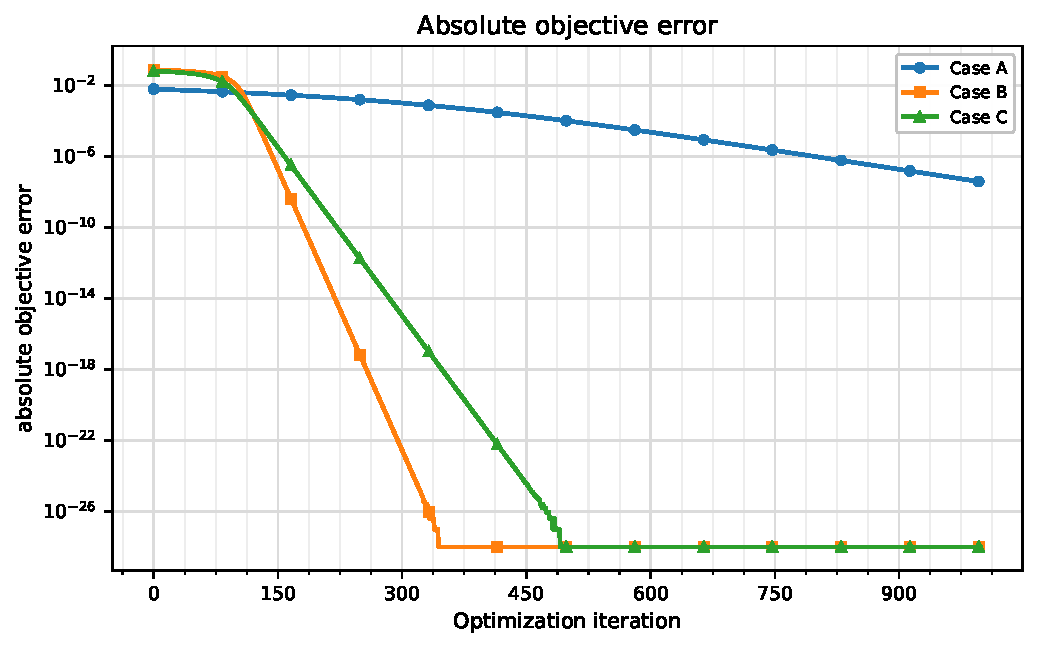
\includegraphics[width=0.86\textwidth]{figures/optimization_objectives.pdf}
  \caption{Absolute zero-target objective error,
  \(|J(u^{(m)})-J_\ast|\) with \(J_\ast=0\), for the three fixed-topology
  examples in Table~\ref{tab:optimization-cases}.  The optimized cost is
  \(J=\frac12|r|^2\), so convergence corresponds to the curves reaching zero.
  Exact zeros are drawn at a small plotting floor on the logarithmic axis.}
  \label{fig:optimization-objectives}
\end{figure}

Figure~\ref{fig:optimization-growth-rates} shows the change in the growth-rate
diagnostics used to form the objectives.  Plotting
\(\gamma^{(m)}-\gamma^{(0)}\) avoids hiding the optimization signal behind the
large offset between initially positive and initially negative cases.  For
cases A and B, the selected and maximum nonzonal rates coincide for the chosen
\(k_y\) grids, so each is shown as a single selected=max curve.  Case C
optimizes the maximum over the two nonzonal modes, while the selected
\(k_y=0.25\) diagnostic is also recorded.

\begin{figure}[htbp]
  \centering
  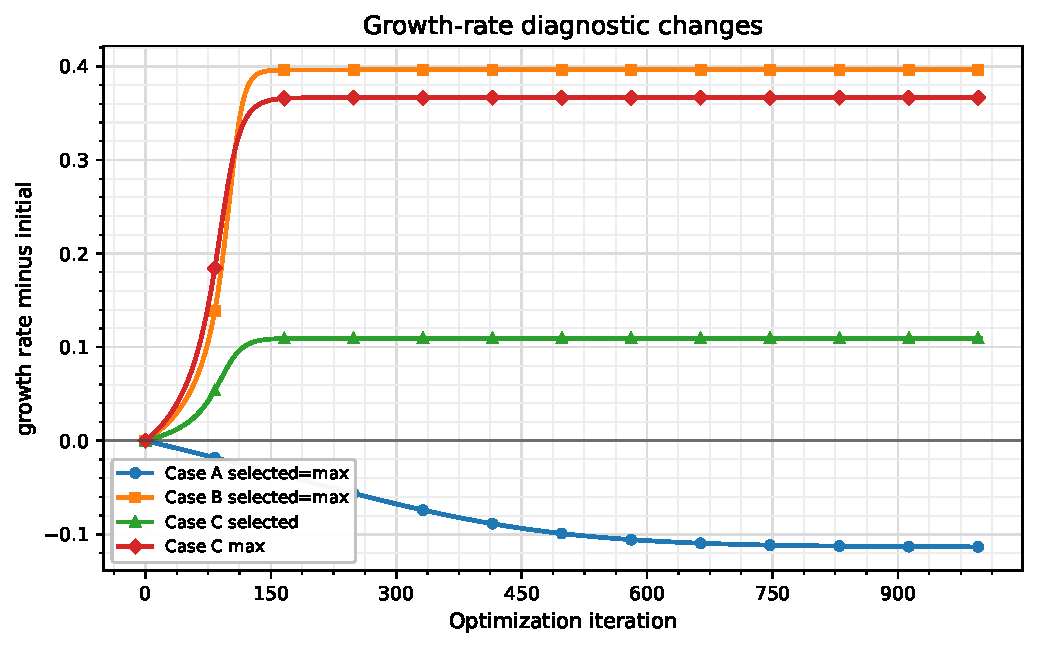
\includegraphics[width=0.86\textwidth]{figures/optimization_growth_rates.pdf}
  \caption{Selected and maximum nonzonal growth-rate changes during the
  reduced optimization runs.  The diagnostic is computed from the potential
  amplitude over the connected \(k_x\)-chain, as in
  Eq.~\eqref{eq:growth-rate}.}
  \label{fig:optimization-growth-rates}
\end{figure}

Figure~\ref{fig:optimization-geometry-knobs} shows the changes in the
continuous geometry knobs \(q\) and \(\hat s\) during the same optimization
runs.  The integer grid, Fourier topology, and mode connectivity are held
fixed; only continuous parameters are differentiated and updated.

\begin{figure}[htbp]
  \centering
  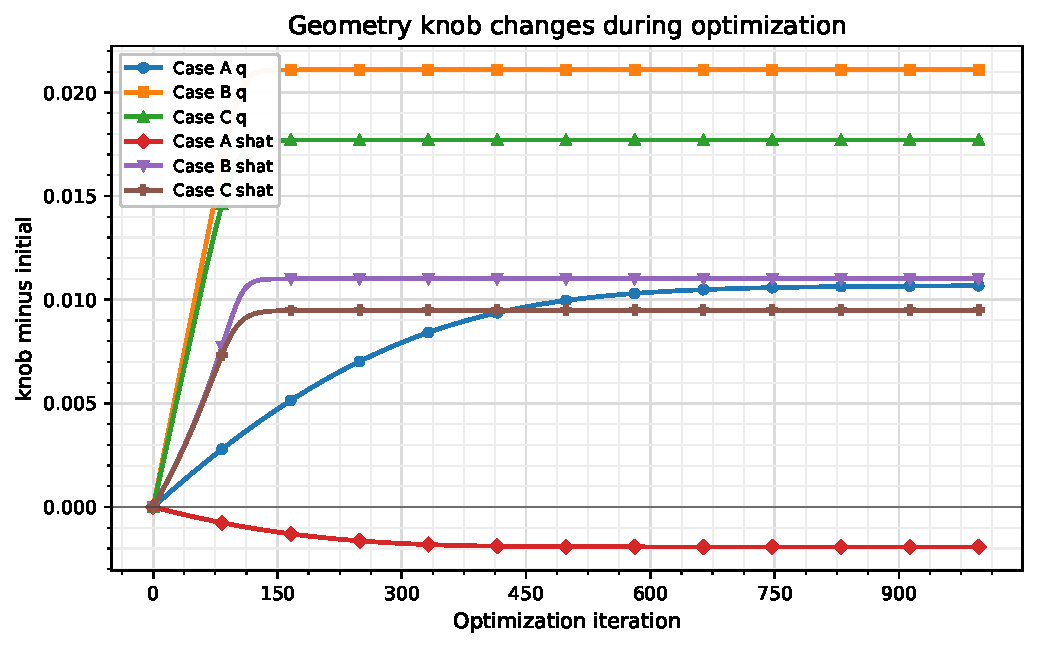
\includegraphics[width=0.86\textwidth]{figures/optimization_geometry_knobs.pdf}
  \caption{Changes in \(q\) and magnetic shear \(\hat s\) under the toy
  gradient-descent updates.  Plotting increments relative to the initial values
  makes the small continuous updates visible while the integer grid and
  mode-connectivity maps remain static.}
  \label{fig:optimization-geometry-knobs}
\end{figure}

The current result should be interpreted narrowly: it is evidence that the
optimization interface is wired through the solver and differentiates through a
fixed number of time steps.  The next physical validation step is to replace the
toy circular-geometry coefficient modulation with DESC-generated flux-tube
fixtures using the imported-array path, and to optimize only after the
Rosenbluth-Hinton, Cyclone Base Case, and GX/eik benchmark checks are stable.

\section{Nonlinear and Extended Physics Roadmap}
\label{sec:nonlinear-extension}

The nonlinear ExB term retained for later is
\begin{equation}
  \mathcal{T}_{III,s}
  =
  -\left\{J_{0,s}\phi,f_s\right\},
  \qquad
  \{a,b\}
  =
  \partial_x a\,\partial_y b-\partial_y a\,\partial_x b.
  \label{eq:nonlinear-bracket}
\end{equation}
The implementation should be pseudospectral:
\begin{enumerate}
  \item multiply by \(\ii k_x\) and \(\ii k_y\) in Fourier space;
  \item inverse FFT to a dealiased real grid;
  \item compute the bracket in real space;
  \item FFT back and truncate to the retained spectral grid.
\end{enumerate}
This is not required for the first linear solver.

Other extensions should be added only after the linear electrostatic baseline is validated:
\begin{itemize}
  \item kinetic electrons via \eqref{eq:phi-kinetic};
  \item collisions from \path{collisionop.F90};
  \item electromagnetic \(A_\parallel\) and \(B_\parallel\);
  \item toroidal rotation and ExB shear from \path{rotation.F90};
  \item nonlinear heat-flux objectives.
\end{itemize}

\section{Implementation and Test Plan}

Every public function in \path{src/} must have a matching unit test.  The intended order is:
\begin{enumerate}
  \item Package skeleton and immutable PyTree parameter types.
  \item Perpendicular Fourier grids plus spectral \(z,\vpar,\mu\) collocation, quadrature, derivative matrices, and filters.
  \item Optional GKW finite-difference backend behind the same derivative interface.
  \item Mode connectivity and static topology maps.
  \item Circular and \(s\)-alpha analytic geometry.
  \item Boozer/stellarator geometry adapter, including DESC-style sampled arrays.
  \item Bessel, \(\Gzero\), Maxwellian, and drive factors.
  \item Adiabatic \(\phi\) solve with separate zonal tests.
  \item Individual RHS term functions.
  \item Full residual \(\RHS\).
  \item RK4 step and growth-rate diagnostics.
  \item Quasilinear objective and gradient checks.
\end{enumerate}

\subsection{Unit tests}

\begin{longtable}{p{0.28\textwidth}p{0.62\textwidth}}
\toprule
Component & Required tests \\
\midrule
Parameter PyTrees & flatten/unflatten, static/dynamic field behavior, JIT compatibility. \\
Grids & shapes, centering, spectral quadrature weights, \(k_x=0\), \(k_y=0\), Parseval weights. \\
Spectral operators & manufactured derivative convergence in \(z\), \(\vpar\), and \(\mu\); modal filter behavior; finite-difference fallback parity on small grids. \\
Mode connectivity & zonal periodic identity, nonzonal chain labels, invalid open ends, GKW sample parity. \\
Geometry & finite values, \(\kperp^2\ge0\), circular/Gyaradax parity, AD gradients vs finite differences. \\
Bessel/polarization & small-argument limits, finite large-argument behavior, AD gradients. \\
Maxwellian/drive & normalization shape, positivity, gradient-drive broadcasting. \\
Phi solve & zero-input invariance, quasineutrality residual, no-zonal and zonal paths, Gyaradax parity. \\
RHS terms & zero-input behavior, linearity in \(f\) where applicable, spectral and fallback manufactured derivative tests. \\
RK4 & scalar ODE order test, zero-input invariance, short-run JIT and gradient checks. \\
Diagnostics & amplitude chain selection, growth-rate recovery, frequency sign convention. \\
Objectives & finite values, smooth gradients, finite-difference agreement on tiny grids. \\
\bottomrule
\end{longtable}

\subsection{Benchmark ladder}

\begin{enumerate}
  \item Tiny manufactured cases: no physics, known derivative, known ODE.
  \item Reduced GKW samples: \path{simple_example}, \path{simple_itg}, and selected \path{cyclone} inputs.
  \item Gyaradax circular and \(s\)-alpha parity tests.
  \item Rosenbluth-Hinton zonal-flow residual.
  \item Cyclone Base Case linear ITG growth rate.
  \item Boozer/DESC geometry fixture: compare \(B\), metric, drift coefficients, and \(\avg{\kperp^2}\).
  \item Stellarator ITG scans over \(\rho,\alpha,k_y\), compared to available GS2/GX/GKW-style references.
\end{enumerate}

\subsection{Done criteria for first solver}

The first solver milestone is complete when:
\begin{itemize}
  \item \(\Phi(f)\), \(\RHS(f)\), RK4 stepping, \(\gamma\), \(\omega\), and \(Q_{\mathrm{QL}}\) are implemented;
  \item all public functions have tests;
  \item a circular/s-alpha ITG benchmark matches the selected reference tolerance;
  \item a Boozer/stellarator geometry fixture runs through the residual and diagnostics;
  \item gradients of \(Q_{\mathrm{QL}}\) with respect to at least \(\omega_T,\omega_n,q,\hat s\), and continuous geometry arrays are finite and finite-difference checked on a reduced grid;
  \item \path{STATUS.md} records commands, tolerances, and remaining caveats.
\end{itemize}

\begin{thebibliography}{9}

\bibitem{peeters2009gkw}
A.~G. Peeters, Y. Camenen, F.~J. Casson, W.~A. Hornsby, A.~P. Snodin, D. Strintzi, and G. Szepesi.
\newblock The nonlinear gyro-kinetic flux tube code GKW.
\newblock \emph{Computer Physics Communications}, 180:2650--2672, 2009.

\bibitem{gyaradax}
G. Galletti, E. Volkmann, and J. Brandstetter.
\newblock \texttt{gyaradax}: local gyrokinetics JAX code.
\newblock Project materials in \path{papers/gyaradax-paper/} and \path{relevant-codes/gyaradax/}.

\bibitem{jorge2024}
R. Jorge, W. Dorland, P. Kim, M. Landreman, N.~R. Mandell, G. Merlo, and T. Qian.
\newblock Direct microstability optimization of stellarator devices.
\newblock \emph{Physical Review E}, 110:035201, 2024.

\bibitem{kim2024}
P. Kim et al.
\newblock Optimization of nonlinear turbulence in stellarators.
\newblock \emph{Journal of Plasma Physics}, 90:905900210, 2024.

\end{thebibliography}

\end{document}
